\chapter{New results : Reevaluating the uncertainties in $\bar{B}\rightarrow X_s\gamma$}\label{reevaluating_b_to_x}

As shown in section \ref{sec:Q1Q7_cont}, the moments of the subleading shape function ($g_{17}$) are used to construct phenomenological models for non-local function $h_{17}$. These models were then used in estimating the $Q_{1}^q-Q_{7\gamma}$ contribution to the uncertainty on total rate ($\mathcal{F}_E|_{17}$). The moments of the $h_{17}$ are related to the higher dimensional HQET matrix elements. In sections \ref{sec:SI_mat_decomp} and \ref{sec:SD_mat_decomp} we constructed a general tensor decomposition of these matrix elements up to and including dimension eight. In the following, we will use this general decomposition to relate the higher order moments of $h_{17}$ to nonperturbative HQET parameters. The updated estimates for these HQET parameters are found in \cite{Gambino:2016jkc}. These estimates were obtained using moments of the semileptonic $B$ decay spectra and information based on lowest lying state saturation approximation. Then a global fit was performed to these HQET parameters to estimate them. In our work, we use the information on HQET parameters to estimate the higher order moments of the $h_{17}$ function. Based on these estimates we construct a new model, and use it to better constrain $\mathcal{F}_E|_{17}$ and the SM estimate of the CP asymmetry in $\bar{B}\to X_s\gamma$ decay. 

\section{Moments of the sub-leading shape function $g_{17}$}\label{sec:chap5_moments_g_17}

Equation (\ref{eqn:chapetr3_h_17}) relates the nonlocal function $h_{17}$ to subleading shape function $g_{17}$. Since $g_{17}$ is a function of both $\omega$ and $\omega_1$, we consider three types of moments. They are moments of $g_{17}$ over $\omega_1$ alone, moments over $\omega$ alone and moments over both $\omega$ and $\omega_1$. In the previous sections we derive the general expression for these moments.

\subsection{Moments in $\omega_1$ alone}

Using equation (\ref{eqn:chapter3_suleadinhg_SSf}), we obtain the moments of $g_{17}$ over $\omega_1$ as follows \cite{Gunawardana:2019gep}:
\begin{eqnarray}\label{eqn:chap5_g_17}
&&\langle\omega^0\,\omega_1^k\,g_{17}\rangle\equiv\int^{\bar \Lambda}_{-\infty}d\omega\int^{\infty}_{-\infty}d\omega_1\,\omega_1^k \,g_{17}(\omega,\omega_1,\mu)=\nonumber\\
&=&
(-1)^k\dfrac{1}{2M_B}\langle\bar B| \big(\bar h S_{\bar n}\big)(0)\,
    \nbslash (1+\gamma_5)\,
    i\gamma_\alpha^\perp\bar n_\beta\,
   (i\bar n\cdot \partial)^k \big(S_{\bar n}^\dagger\,g G_s^{\alpha\beta} S_{\bar n} 
    \big)(r\bar n)\,
    \big(S_{\bar n}^\dagger h\big)(0) |\bar B\rangle\big|_{r=0},\nonumber\\
\end{eqnarray}
where $\gamma^{\perp}$ represents only the $\gamma^{1}$ and $\gamma^{2}$, $n=(1,0,0,1)$ and $\bar{n}=(1,0,0,-1)$. The integrals over $\omega$ and $\omega_{1}$, generates the delta functions of $r,t$. These delta functions restricts the evaluation of the matrix element at $r=0,t=0$. Using the identity $i \bar{n} \cdot \partial\left(S_{\bar{n}}^{\dagger}(x) O(x) S_{\bar{n}}(x)\right)=S_{\bar{n}}^{\dagger}(x)[i \bar{n}\cdot D,O(x)]S_{\bar{n}}(x)$, which is proved in appendix \ref{appen_b}, we obtain
\begin{eqnarray}\label{eqn:chap5_Generalw1}
&&\langle\omega^0\,\omega_1^k\,g_{17}\rangle\equiv\int^{\bar \Lambda}_{-\infty}d\omega\int^{\infty}_{-\infty}d\omega_1\,\omega_1^k \,g_{17}(\omega,\omega_1,\mu)=\nonumber\\
&=&(-1)^k\dfrac{1}{2M_B}\langle\bar B| \bar h \,
    \nbslash (1+\gamma_5)\,
    i\gamma_\alpha^\perp\bar n_\beta\,\underbrace{\big[i\bar n\cdot D,\big[i\bar n \cdot D,\cdots[i\bar n \cdot D}_\text{$k$ times},g G_s^{\alpha\beta}\big]\cdots\big]\big] h |\bar B\rangle=\nonumber\\
&=&(-1)^k\dfrac{1}{2M_B}\langle\bar B| \bar h \,
    \nbslash (1+\gamma_5)\,
    \gamma_\alpha^\perp\,\underbrace{\big[i\bar n\cdot D,\big[i\bar n \cdot D,\cdots[i\bar n \cdot D}_\text{$k$ times},\big[iD^\alpha ,i\bar n \cdot D\big]\cdots\big]\big] h |\bar B\rangle.\nonumber\\
\end{eqnarray}
The identity $\big[iD^\mu,iD^\nu\big]=igG^{\mu\nu}$ was used in the last line.\par
The Dirac structures in the matrix elements are simplified using the projection operators $P_{+}$, which are defined in section \ref{sec:def}. As shown in equation (\ref{trans2}), the action of projection operators on $\gamma^{\lambda}\gamma^5$ provides $s^{\lambda}$. Using this we simplify the Dirac structure. For example, consider the term $\slashed{\bar{n}}\gamma_{\alpha}^{\perp}$. The orthogonality between $\alpha$ and $\bar{n}$ provides that $\nbslash\gamma_\alpha^\perp=-i\sigma_{\mu\alpha_\perp}\bar n^\mu$. Equation (\ref{trans3}) provides the relationship between $\sigma_{\mu\alpha}$ and $s^{\lambda}$. Note that we used the convention $\epsilon_{0123}=-1$. As a result, we obtain $\nbslash\gamma_\alpha^\perp\to iv^\rho\epsilon_{\rho\mu\alpha_\perp\lambda}s^\lambda\bar n^\mu$. The Dirac structure $\nbslash\gamma^5\gamma_\alpha^\perp$ is then simplified using equation (\ref{eqn:chap4_matrix_decomp}), which provides $P_+\nbslash\gamma^5\gamma_\alpha^\perp P_+\to-s^{\alpha_\perp}$. Using this we obtain
\begin{eqnarray}\label{eqn:chap5_mom_g17_omega_1}
&&\langle\omega^0\omega_1^kg_{17}\rangle\equiv\int^{\bar \Lambda}_{-\infty}d\omega\int^{\infty}_{-\infty}d\omega_1\,\omega_1^k \,g_{17}(\omega,\omega_1,\mu)=\nonumber\\
&=&\left(iv^\rho\epsilon_{\rho\mu\alpha_\perp\lambda}\bar n^\mu-g_{\alpha_\perp\lambda}\right)(-1)^k\dfrac{1}{2M_B}\langle\bar B| \bar h \,
    \underbrace{\big[i\bar n\cdot D,\big[i\bar n \cdot D,\cdots[i\bar n \cdot D}_\text{$k$ times},\big[iD^\alpha ,i\bar n \cdot D\big]\cdots\big]\big] s^\lambda h |\bar B\rangle,\nonumber\\
\end{eqnarray}

where the parameters $g_\perp^{\mu\nu}$ and $\epsilon_\perp^{\mu\nu}$ are defined in equation (\ref{eqn:Transverse_indices_contract}). The nested commutators in equation (\ref{eqn:chap5_mom_g17_omega_1}) implies that the odd moments of $g_{17}$ over $\omega_1$ vanishes. This is due to the odd number of commutators of Hermitian operators is a Hermitian operator. Thus the corresponding HQET matrix element becomes real. As shown in the chapter \ref{chap:Matrix_elements}, the spin dependent matrix elements are imaginary \cite{Gunawardana:2017zix}. As a result, the real matrix elements obtained from the odd moments in $\omega_1$ must vanish.\par
We use the general decomposition constructed in the sections \ref{sec:SI_mat_decomp} and \ref{sec:SD_mat_decomp} to obtain the moments in $\omega_1$ up to third moment. The moments of $g_{17}$ over $\omega_1$ are listed :
\vspace{-0.3cm}
\begin{eqnarray}\label{eqn:chap5_w1moments}
&&\langle\omega^0\,\omega_1^0\,g_{17}\rangle\equiv\int^{\bar \Lambda}_{-\infty}d\omega\int^{\infty}_{-\infty}d\omega_1\,g_{17}(\omega,\omega_1,\mu)=4\tilde{a}^{(5)}=2\lambda_2=2\mu_G^2/3\nonumber\\
&&\langle\omega^0\,\omega_1^1\,g_{17}\rangle\equiv\int^{\bar \Lambda}_{-\infty}d\omega\int^{\infty}_{-\infty}d\omega_1\,\omega_1 \,g_{17}(\omega,\omega_1,\mu)=0\nonumber\\
&&\langle\omega^0\,\omega_1^2\,g_{17}\rangle\equiv\int^{\bar \Lambda}_{-\infty}d\omega\int^{\infty}_{-\infty}d\omega_1\,\omega_1^2 \,g_{17}(\omega,\omega_1,\mu)=4 \left(-4 \tilde{a}^{(7)}_{12} + 2 \tilde{a}^{(7)}_{13} + 3 \tilde{a}^{(7)}_{14} - \tilde{a}^{(7)}_{23} + \tilde{b}^{(7)}\right)=\nonumber\\
&&=\dfrac2{15} \left(5 m_5 + 3 m_6 - 2 m_9\right)\nonumber\\
&&\langle\omega^0\,\omega_1^3\,g_{17}\rangle\equiv\int^{\bar \Lambda}_{-\infty}d\omega\int^{\infty}_{-\infty}d\omega_1\,\omega_1^3 \,g_{17}(\omega,\omega_1,\mu)=0.
\end{eqnarray}  

The zeroth moment is a known result, and the second moment was first obtained in \cite{Gunawardana:2019gep}.

\subsection{Moments in $\omega$ alone}

The moments of $g_{17}$ over $\omega$ are obtained by evaluating
\vspace{-0.3cm}
\begin{eqnarray}\label{eqn:chap5_Generalw}
&&\langle\omega^k\,\omega_1^0\,g_{17}\rangle\equiv\int^{\bar \Lambda}_{-\infty}d\omega\,\omega^k \int^{\infty}_{-\infty}d\omega_1\,g_{17}(\omega,\omega_1,\mu)=\nonumber\\
&=&\int^{\bar \Lambda}_{-\infty}d\omega\,\omega^k  \int\frac{dt}{2\pi}\,e^{-i\omega t} 
\dfrac{1}{2M_B}\langle\bar B| \big(\bar h S_{n}\big)(tn)\,
    \nbslash (1+\gamma_5)\,S_n^\dagger (0)\,
    i\gamma_\alpha^\perp\bar n_\beta\,
   g G_s^{\alpha\beta}(0)
    h(0) |\bar B\rangle=\nonumber\\
&=&\int^{\bar \Lambda}_{-\infty}d\omega\,\omega^k  \int\frac{dt}{2\pi}\,e^{i\omega t} 
\dfrac{1}{2M_B}\langle\bar B| \big(\bar h S_{n}\big)(0)\,
    \nbslash (1+\gamma_5)\,S_n^\dagger (tn)\,
    i\gamma_\alpha^\perp\bar n_\beta\,
   g G_s^{\alpha\beta}(tn)
    h(tn) |\bar B\rangle=\nonumber\\
&=&\int\,dt\,\delta(t)
\dfrac{1}{2M_B}\langle\bar B|\bar h(0) S_{n}(0)\,(in\cdot\partial)^kS_n^\dagger (tn)\,
    \nbslash (1+\gamma_5)\,
    i\gamma_\alpha^\perp\bar n_\beta\,
   g G_s^{\alpha\beta}(tn)
    h(tn) |\bar B\rangle.
        \end{eqnarray}

In the above expression we used the transnational invariace of nonlocal matrix elements along $n$. Using the identity $S_{n}^\dagger(tn)\,in\cdot D\,=in\cdot \partial \,S^\dagger_n(tn)$ we obtain a general expression for the moments over $\omega$:

\begin{eqnarray}
&&\langle\omega^k\,\omega_1^0\,g_{17}\rangle\equiv\int^{\bar \Lambda}_{-\infty}d\omega\,\omega^k \int^{\infty}_{-\infty}d\omega_1\,g_{17}(\omega,\omega_1,\mu)=\nonumber\\
&=&\left(iv^\rho\epsilon_{\rho\mu\alpha_\perp\lambda}\bar n^\mu-g_{\alpha_\perp\lambda}\right)\dfrac{1}{2M_B}\langle\bar B| \bar h \,
   \left(in \cdot D\right)^k\big[iD^\alpha ,i\bar n \cdot D\big]s^\lambda h |\bar B\rangle.\nonumber\\
\end{eqnarray}

We used the general decomposition defined in sections \ref{sec:SI_mat_decomp} and \ref{sec:SD_mat_decomp} to obatin the moments up to and including $\left\langle\omega^{3} \omega_{1}^{0} g_{17}\right\rangle$.

\begin{eqnarray}
&&\langle\omega^0\,\omega_1^0\,g_{17}\rangle\equiv\int^{\bar \Lambda}_{-\infty}d\omega\int^{\infty}_{-\infty}d\omega_1\,g_{17}(\omega,\omega_1,\mu)=4\tilde{a}^{(5)}=2\lambda_2=2\mu_G^2/3\nonumber\\
&&\langle\omega^1\,\omega_1^0\,g_{17}\rangle\equiv\int^{\bar \Lambda}_{-\infty}d\omega\,\omega\int^{\infty}_{-\infty}d\omega_1 \,g_{17}(\omega,\omega_1,\mu)=-2\tilde{a}^{(6)}=-\rho_2=-\rho^3_{LS}/3\nonumber\\
&&\langle\omega^2\,\omega_1^0\,g_{17}\rangle\equiv\int^{\bar \Lambda}_{-\infty}d\omega\,\omega^2\int^{\infty}_{-\infty}d\omega_1 \,g_{17}(\omega,\omega_1,\mu)=-2 \left(2 \tilde{a}^{(7)}_{12} - \tilde{a}^{(7)}_{14} +  \tilde{a}^{(7)}_{23} + \tilde{b}^{(7)}\right)=\nonumber\\
&&=-\dfrac1{60} \left(20 m_5 +2 m_7 + m_8\right)\nonumber\\
&&\langle\omega^3\,\omega_1^0\,g_{17}\rangle\equiv\int^{\bar \Lambda}_{-\infty}d\omega\,\omega^3\int^{\infty}_{-\infty}d\omega_1 \,g_{17}(\omega,\omega_1,\mu)=\nonumber\\
&&=-2 \left(2 \tilde{a}^{(8)}_{12} - \tilde{a}^{(8)}_{15} +  \tilde{a}^{(8)}_{24} +2 \tilde{b}^{(8)}_{13} + \tilde{b}^{(8)}_{14} - \tilde{b}^{(8)}_{15} - 2\tilde{b}^{(8)}_{35} - \tilde{b}^{(8)}_{45} + \tilde{c}^{(8)}\right)=\nonumber\\
&&=-\dfrac1{15} \left(5r_8 - r_9 +2 r_{10}+r_{11}-2r_{12}-r_{13}+2r_{15}-r_{16}+r_{17}\right)\nonumber\\
\end{eqnarray}  

\vspace{0.2cm}
The first moment was derived in \cite{Benzke:2010js}, and the third and fourth moments were first derived in \cite{Gunawardana:2019gep}.

\subsection{Moments in both $\omega_1$ and $\omega$}

General expression for mixed moments of $g_{17}$ over $\omega$ and $\omega_1$ can be obtained as follows:

\begin{eqnarray}\label{eqn:chap5_Generalww1}
&&\langle\omega^l\,\omega_1^k\,g_{17}\rangle\equiv\int^{\bar \Lambda}_{-\infty}d\omega\,\omega^l \int^{\infty}_{-\infty}d\omega_1\,\omega^k\,g_{17}(\omega,\omega_1,\mu)=\left(iv^\rho\epsilon_{\rho\mu\alpha_\perp\lambda}\bar n^\mu-g_{\alpha_\perp\lambda}\right)(-1)^k\times\nonumber\\
&\times&\dfrac{1}{2M_B}\langle\bar B| \bar h \,(i n\cdot D)^l
    \underbrace{\big[i\bar n\cdot D,\big[i\bar n \cdot D,\cdots[i\bar n \cdot D}_\text{$k$ times},\big[iD^\alpha ,i\bar n \cdot D\big]\cdots\big]\big] s^\lambda h |\bar B\rangle.
\end{eqnarray} 

Using the tesnor decomposition of HQET matrix elements we found the mixed moments of $\omega$ and $\omega_1$ up to dimension eight matrix elements. They are :

\begin{eqnarray}
&&\langle\omega^1\,\omega_1^1\,g_{17}\rangle\equiv\int^{\bar \Lambda}_{-\infty}d\omega\,\omega\int^{\infty}_{-\infty}d\omega_1\,\omega_1 \,g_{17}(\omega,\omega_1,\mu)=2 \left(-4 \tilde{a}^{(7)}_{12}+ 2\tilde{a}^{(7)}_{13} +3 \tilde{a}^{(7)}_{14} -  \tilde{a}^{(7)}_{23} + \tilde{b}^{(7)}\right)=\nonumber\\
&&=\dfrac1{15} \left(5 m_5 +3 m_6 -2m_9\right)\nonumber\\
%
&&\langle\omega^2\,\omega_1^1\,g_{17}\rangle\equiv\int^{\bar \Lambda}_{-\infty}d\omega\,\omega^2\int^{\infty}_{-\infty}d\omega_1\,\omega_1 \,g_{17}(\omega,\omega_1,\mu)=\nonumber\\
&&=2 \left(3 \tilde{a}^{(8)}_{12} - \tilde{a}^{(8)}_{14}  -2\tilde{a}^{(8)}_{15} +  \tilde{a}^{(8)}_{24} -3 \tilde{b}^{(8)}_{13} + \tilde{b}^{(8)}_{14} +4\tilde{b}^{(8)}_{15} +3\tilde{b}^{(8)}_{35} - \tilde{b}^{(8)}_{45} + \tilde{c}^{(8)}\right)=\nonumber\\
&&=\dfrac1{15} \left(5r_8 - r_9 -3 r_{10}+r_{11}+3r_{12}+4r_{13}+3r_{15}-2r_{16}+r_{17}-r_{18}\right)\nonumber\\
%
&&\langle\omega^1\,\omega_1^2\,g_{17}\rangle\equiv\int^{\bar \Lambda}_{-\infty}d\omega\,\omega^1\int^{\infty}_{-\infty}d\omega_1\,\omega_1^2 \,g_{17}(\omega,\omega_1,\mu)=\nonumber\\
&&=2 \left(3 \tilde{a}^{(8)}_{12} - \tilde{a}^{(8)}_{14} - 2\tilde{a}^{(8)}_{15} +  \tilde{a}^{(8)}_{24} +3 \tilde{b}^{(8)}_{13} + \tilde{b}^{(8)}_{14} - 2\tilde{b}^{(8)}_{15} + 2\tilde{b}^{(8)}_{34} -\tilde{b}^{(8)}_{35} + \tilde{b}^{(8)}_{45} - \tilde{c}^{(8)}\right)=\nonumber\\
&&=\dfrac1{15} \left(-5r_8 + r_9 +3 r_{10}+r_{11}-r_{12}-2r_{13}+2r_{14}+3r_{15}-2r_{16}+r_{17}-r_{18}\right)
\end{eqnarray}  
These moments were all first obtained in \cite{Gunawardana:2019gep}. 

\section{Applications}

\subsection{Estimating the moments of subleading shape function}

As shown in the section \ref{sec:chap5_moments_g_17}, the moments of the subleading shape function are related to nonperturbative HQET parameters. In \cite{Gambino:2016jkc} the numerical estimates for these HQET parameters were provided up to and including dimension eight. For this, the moments of the semileptonic $B$ decay spectra and lowest lying saturation approximation (LLSA) were used \cite{Mannel:2010wj,Heinonen:2014dxa}. Using the LLSA the higher dimensional matrix elements were related to the lower dimensional matrix elements and to the excitation energy $\epsilon$ \cite{Gambino:2016jkc}. This approximation provides $50-100\%$ accuracy \cite{Heinonen:2014dxa}. Based on the central values and the standard deviation provided in the table $2$ of \cite{Gambino:2016jkc} we obtain the moments of the $g_{17}$ as follows:

\begin{eqnarray}\label{eqn:chap5_moments_numerical}
\langle\omega^0\,\omega_1^0\,g_{17}\rangle&=&0.237\pm0.040 \mbox{ GeV}^2\nonumber\\
\langle\omega^0\,\omega_1^2\,g_{17}\rangle&=&0.15\pm0.12 \mbox{ GeV}^4\nonumber\\
\langle\omega^1\,\omega_1^0\,g_{17}\rangle&=&0.056\pm0.032 \mbox{ GeV}^3\nonumber\\
\langle\omega^2\,\omega_1^0\,g_{17}\rangle&=&0.015\pm0.021 \mbox{ GeV}^4\nonumber\\
\langle\omega^3\,\omega_1^0\,g_{17}\rangle&=&0.008\pm0.011 \mbox{ GeV}^5\nonumber\\
\langle\omega^1\,\omega_1^1\,g_{17}\rangle&=&0.073\pm0.059 \mbox{ GeV}^4\nonumber\\
\langle\omega^2\,\omega_1^1\,g_{17}\rangle&=&-0.034\pm0.016 \mbox{ GeV}^5\nonumber\\
\langle\omega^1\,\omega_1^2\,g_{17}\rangle&=&0.027\pm0.014 \mbox{ GeV}^5,
\end{eqnarray}  
The errors of the HQET parameters were added in the quadrature. In \cite{Gambino:2016jkc} the errors of the HQET parameters were reported without the correlated error. Therefore, in our work we did not consider the correlated error as well. \par
Even though the relative errors of these nonperturbative parameters are large, they still provide useful information regarding the moments of the subleading shape function. For example, using the model provided in \cite{Benzke:2010js} for $h_{17}$ we found that $\langle\omega^0\,\omega_1^2\,g_{17}\rangle\in [-0.31,0.49]\text{ GeV}^4$. This should be compared to the $\langle\omega^0\,\omega_1^2\,g_{17}\rangle = 0.15\pm0.12 \mbox{ GeV}^4$ in equation (\ref{eqn:chap5_moments_numerical}). The range of $\langle\omega^0\,\omega_1^2\,g_{17}\rangle$ found in \cite{Benzke:2010js} is roughly three times bigger compared to the new one.\par
The nonperturbative HQET parameters that are defined in \cite{Mannel:2010wj} and listed in \cite{Gambino:2016jkc} used the full QCD $b$ fields. Whereas, the HQET matrix elements are defined in heavy quark limit. As a result, there is a $1/m_b$ difference between the parameters defined in these two basis. For instance, the relation between $\lambda_2$ and $\mu_G^2$ contains a $1/m_b$ correction term. However, this difference is not numerically important. This is due to the relatively large error bars in our moment estimates. To illustrate this further, consider the value of $\mu_G^2/3$ obtained in \cite{Gambino:2016jkc}. We compare this estimate of $\mu_G^2/3$ to the $\lambda_2$, which is extracted from the $B$ and $D$ meson spectroscopy. Note that the value of $\lambda_2$ is defined in the heavy quark limit.\par
\begin{figure}
\begin{center}
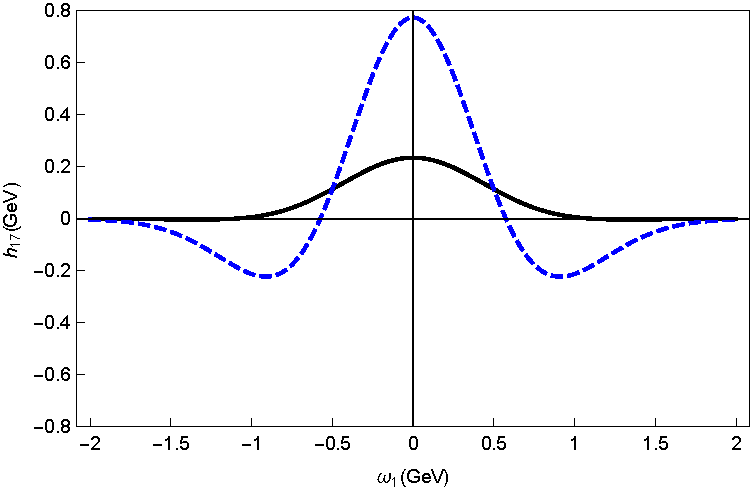
\includegraphics[scale=0.6]{FigureMoment2Low.pdf}
\hspace{1cm}
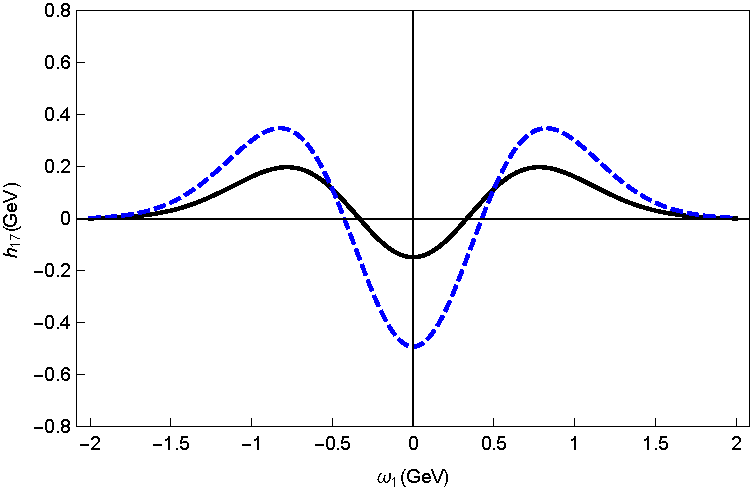
\includegraphics[scale=0.6]{FigureMoment2High.pdf}
\caption{\label{fig1} A comparison of the extremal models for $h_{17}$ as a sum of two lowest even Hermite polynomials times a Gaussian of width $0.5$ GeV used in \cite{Benzke:2010js} (dashed blue) to the same models allowed by current (2019) data (solid black). Left hand side:  The model with 2010 smallest possible second moment of $-0.31\mbox{ GeV}^4$ compared to 2019 smallest possible second moment of $0.03\mbox{ GeV}^4$. Right hand side:  The model with 2010 largest possible second moment of $0.49\mbox{ GeV}^4$ compared to 2019 largest possible second moment of $0.27\mbox{ GeV}^4$. 
}
\end{center}
\end{figure}
We define the mass split as $\Delta m_H=m_H^*-m_H$, where $m_H$ is a pseudo-scalar and $m_H^*$ is vector heavy meson containing a heavy quark of mass $m_Q$. 
At order $1/m_b$ the $\lambda_2=\Delta m_Hm_H/2$. We extractred the value of $\lambda_2$ using the isospin-averaged meson mass data \cite{Tanabashi:2018oca}. Following from this, we obtain $\lambda_2=0.119\pm 0.001\mbox{ GeV}^2$ for $B$ meson data. For the $D$ meson data we obtain $\lambda_2=0.13193\pm0.00002\mbox{ GeV}^2$ \cite{Gunawardana:2019gep}.\par
At order $\mathcal{O}(1/m_b^2)$ the expression for $\lambda_2$ is \cite{Gremm:1996df}
\begin{eqnarray}\label{eqn:chap5_l2_O_m_2}
\lambda_{2}\left(m_{b}\right)=\frac{\Delta m_{B} m_{B}^{2}-\Delta m_{D} m_{D}^{2}}{2\left(m_{B}-\kappa\left(m_{c}\right) m_{D}\right)}
\end{eqnarray} 
Equation (\ref{eqn:chap5_l2_O_m_2}) provides $\lambda_2=0.112\pm 0.001\mbox{ GeV}^2$. In comparison, $\mu_G^2/3=0.118\pm 0.020\mbox{ GeV}^2$  \cite{Gambino:2016jkc} is equal to all these values of $\lambda_2$ within the error. As a result, it is currently not possible to distinguish between $\lambda_2$ and $\mu_G^2$. Hence, in the following work we use $\mu_G^2/3$ from \cite{Gambino:2016jkc}, and we assume a similar behavior for all other HQET parameters. This situation can be improved with the availability of the future Belle II data and Lattice QCD. These new data can improve the estimates of HQET parameters and the moments. 

\subsection{Resolved photon contributions for $Q^q_1-Q_{7\gamma}$}

In the following work, we will use the moments of subleading shape function to better constrain the resolved photon contributions from the $Q_1^q-Q_{7\gamma}$. As shown in \cite{Benzke:2010js} the contribution from $Q^u_1-Q_{7\gamma}$ vanishes. The contribution from $Q^c_1-Q_{7\gamma}$ is given by

\begin{equation}\label{F17def}
{\cal F}^{17}_E = \frac{C_1(\mu)}{C_{7\gamma}(\mu)}\,\frac{\Lambda_{17}(m_c^2/m_b,\mu)}{m_b},
\end{equation}
where the nonperturbative quantity $\Lambda_{17}$ is defined in equation (\ref{eqn:chapter3_soft_functions}), and it depends on non-local forward scattering matrix element $h_{17}$. Since the $h_{17}$ cannot be obtained from first principles, we use its moments to construct a phenomenological model to describe $h_{17}$. Using the general decomposition provided in sections \ref{sec:SI_mat_decomp}, \ref{sec:SD_mat_decomp} and the numerical estimates of HQET parameters found in \cite{Gambino:2016jkc} we construct new model to better constraint ${\cal F}^{17}_E$.\par
The $Q^q_1-Q_{7\gamma}$ part of the resolved photon contribution to the estimate of CP asymmetry is given in equation (\ref{eqn:resolved_p_cont_CP}). This contribution is defined by the nonperturbative parameters $\tilde{\Lambda}^u_{17}$ and $\tilde{\Lambda}^c_{17}$. With the new information on the moments of subleading shape function $h_{17}$ we would like to revisit the evaluation of these nonperturbative parameters. In addition, we consider the uncertainty generated in evaluation of charm and bottom quark masses.
\vspace{-0.3cm}
\subsubsection{Uncertainty due to the running quark masses}
\vspace{-0.2cm}
For the evaluation of CP averaged rate we use the $m_c = m_c(\mu)$ defined in the $\overline{\mbox{MS}}$ scheme with $\mu=1.5$ GeV. Whereas, the evaluation of CP asymmetry is carried out by using $m_c = m_c(\mu)$ defined in the $\overline{\mbox{MS}}$ scheme with $\mu=2.0$ GeV.\par
The running of the quark masses is given as \cite{Buras:1998raa}
\vspace{-0.4cm}
\begin{eqnarray}\label{eqn:chap5_running_mass}
m(\mu)=m\left(\mu_{0}\right)\left[\frac{\alpha_{s}(\mu)}{\alpha_{s}\left(\mu_{0}\right)}\right]^{\frac{\gamma_{m}^{(0)}}{2 \beta_{0}}}\left[1+\left(\frac{\gamma_{m}^{(1)}}{2 \beta_{0}}-\frac{\beta_{1} \gamma_{m}^{(0)}}{2 \beta_{0}^{2}}\right) \frac{\alpha_{s}(\mu)-\alpha_{s}\left(\mu_{0}\right)}{4 \pi}\right],
\end{eqnarray}

where $\alpha_s, v(\mu), \gamma_m^{0,1}$, and $ \beta_{0,1}$ are given by

\begin{eqnarray}
\alpha_{s}(\mu)=\frac{\alpha_{s}\left(M_{Z}\right)}{v(\mu)}\left[1-\frac{\beta_{1}}{\beta_{0}} \frac{\alpha_{s}\left(M_{Z}\right)}{4 \pi} \frac{\ln v(\mu)}{v(\mu)}\right],
\end{eqnarray}
and 
\begin{align}
&v(\mu)=1-\beta_{0} \frac{\alpha_{s}\left(M_{Z}\right)}{2 \pi} \ln \left(\frac{M_{Z}}{\mu}\right)\nonumber\\
&\gamma_{m}\left(\alpha_{s}\right)=\gamma_{m}^{(0)} \frac{\alpha_{s}}{4 \pi}+\gamma_{m}^{(1)}\left(\frac{\alpha_{s}}{4 \pi}\right)^{2}\nonumber\\
&\beta_{0,1}\left(\alpha_{s}\right)=a_{1} \frac{\alpha_{s}}{4 \pi}+a_{2}\left(\frac{\alpha_{s}}{4 \pi}\right)^{2}\nonumber \\ 
&\gamma_{m}^{(0)}=6 C_{F} \qquad \gamma_{m}^{(1)}=C_{F}\left(3 C_{F}+\frac{97}{3} N-\frac{10}{3} f\right)
\end{align}

$C_{F}=\frac{N^{2}-1}{2 N}$, where $N$ is the number of color charges, and $f$ is the number of effective flavors. In the 2019 update of the 2018 PDG listing we found $m_c(\,m_c)=1.27\pm0.02$ GeV \cite{Tanabashi:2018oca}. The coupling constant is given by $\alpha_s(\mu=m_c) = 0.38 \pm0.03$ \cite{Tanabashi:2018oca}. Using these values and equation (\ref{eqn:chap5_running_mass}) we obtain $m_c(1.5 \mbox{ GeV})=1.20\pm0.03$ GeV and $m_c(2.0 \mbox{ GeV})=1.10\pm0.03$ GeV.\par
In \cite{Benzke:2010js} the estimate of $\Lambda_{17}$ was obtained by using the $m_c = 1.131$ GeV. This charm quark mass is based on smaller vale of $m_c(m_c)$ \cite{Hoang:2005zw}, and it was used in \cite{Misiak:2006zs,Misiak:2006ab} as well. This change in the charm mass tends to slightly affect the estimates of $\Lambda_{17}, \tilde{\Lambda}_{17}^c$.\par
The mass of the bottom quark is obtained by using the shape function scheme \cite{Benzke:2010js,Bosch:2004th}. The updated HFLAG \cite{Amhis:2016xyh} value of $m_b$ is $4.58\pm0.03$ GeV. This value should be compared to the $m_b = 4.65$ GeV used in \cite{Benzke:2010js}.
\vspace{-0.3cm}
\subsubsection{$\Lambda_{17}$ estimates based on expanded penguin function}
\vspace{-0.2cm}
As shown in the equation (\ref{eqn:chapter3_soft_functions}), the soft function $h_{17}$, which appears in the expression of $\Lambda_{17}$, is convoluted with the penguin function ($F(x)$), where $F$ is defined in equation (\ref{eqn:chapter3_penguin_fn}). The expansion of the $1-F(x)$ is given in equation (\ref{eqn:chapter3_F_expansion}), which is obtained for $x>1/4$.\par
In the region $\omega_1\ll 4m^2_c/m_b\approx 1.2-1.3$ GeV we can expand the $F(x)$ and obtain the $\Lambda_{17}$ in terms of moments of the subleading shape function. Starting from the expression of $\Lambda_{17}$ \cite{Benzke:2010js}
\begin{eqnarray}\label{eqn:chap5_L17power}
   \Lambda_{17}\Big(\frac{m_c^2}{m_b},\mu\Big)
   &=& e_c\,\mbox{Re} \int_{-\infty}^{\bar\Lambda}\!d\omega
    \int_{-\infty}^\infty \frac{d\omega_1}{\omega_1} \nonumber\\
   &\quad\times& \left\{ \left( \frac{m_b+\omega}{m_b} \right)^3 
    \left[ 1 - F\!\left( \frac{m_c^2-i\varepsilon}{(m_b+\omega)\,\omega_1} \right) \right]
    + \frac{m_b\,\omega_1}{12m_c^2} \right\} g_{17}(\omega,\omega_1,\mu) \,.
\end{eqnarray}
Using the definition of $h_{17}$ we have $\langle\omega^0\,\omega_1^k\,g_{17}\rangle=\langle\omega_1^k\,h_{17}\rangle$. Then the expansion of the penguin function provides \cite{Gunawardana:2019gep}:
\begin{equation}\label{eqn:chap5_Lambda17expanded}
\Lambda_{17}^{\mbox{\scriptsize expanded}}=  -\dfrac{e_c m_b^3}{560\,m_c^6} \langle\omega^0\,\omega_1^2\,g_{17}\rangle+\cdots=-6\pm5\mbox{ MeV}+\cdots,
\end{equation}

where $\cdots$ denotes the contributions from the higher order moments over $\omega_1$. Traditionally, the contribution from the zeroth moment in $\omega_1$ is subtracted  in equations (\ref{eqn:chapter3_soft_functions}) and (\ref{eqn:chap5_L17power}), and its magnitude is $-e_cm_b2\lambda_2/(12m_c^2)=-42\pm7 \mbox{ MeV}$. The contributors to the uncertainty in the equation (\ref{eqn:chap5_Lambda17expanded}) are $\langle\omega^0\,\omega_1^2\,g_{17}\rangle$, $m_b$, and $m_c$. These uncertainties were added in quadrature.\par
In the past, the size of the contribution from higher operators was a concern for the authors in \cite{Voloshin:1996gw, Ligeti:1997tc, Grant:1997ec, Buchalla:1997ky}. They have noticed the numerical suppression arising from the expansion of the penguin function \cite{Gunawardana:2019gep}. They have noticed the numerical suppression arising from the expansion
of the penguin function, but the lack of knowledge of the matrix elements prevented
them from making conclusive statements.\par
The first term in the equation (\ref{eqn:chapter3_F_expansion}) is suppressed by a factor $\sim 50$ compared to the third term. However, when the third term is combined with the second moment, we obtain  $-6\mbox{ MeV}$. This is only suppressed by a factor of $7$ compared to the zeroth moment. This smaller suppression is consistent with the power counting of $m_c^2\sim m_b\Lambda_{\mbox{\scriptsize QCD}}$, which disfavors the expansion of the penguin function \cite{Gunawardana:2019gep}.\par
Consider the $1/m^n_b$ corrections to $\Lambda_{17}^{\mbox{\scriptsize expanded}}$, which are obtained by expansion of $F(x)$ in $\omega/m_b$. By definition, $\Lambda_{17}^{\mbox{\scriptsize expanded}}=\delta \Lambda_{17}^{(0)}$. For $\delta\Lambda_{17}^{(1)}$ we have  \cite{Gunawardana:2019gep}:

\begin{eqnarray}\label{eqn:chapter5_dLamda_17_1}
\delta \Lambda_{17}^{(1)}&=& -\dfrac{e_c}{3\,m_c^2} \langle\omega^1\,\omega_1^0\,g_{17}\rangle-\dfrac{e_cm_b}{18\,m_c^4} \langle\omega^1\,\omega_1^1\,g_{17}\rangle-\dfrac{3e_cm_b^2}{280\,m_c^6} \langle\omega^1\,\omega_1^2\,g_{17}\rangle+\cdots\nonumber\\
&=&\left(-9\pm5\mbox{ MeV}\right)+\left(-6\pm5\mbox{ MeV}\right)+\left(-1\pm1\mbox{ MeV}\right)+\cdots=-16\pm7\mbox{ MeV}+\cdots\,.\nonumber\\ 
\end{eqnarray}

Again in the equation (\ref{eqn:chapter5_dLamda_17_1}), we observe a slow convergence. Only in the third term we see a suppression compared to the first two terms. Although $\delta \Lambda_{17}^{(1)}$ is a $\Lambda_{\mbox{\scriptsize QCD}}/m_b$ correction, equation (\ref{eqn:chapter5_dLamda_17_1}) indicates that the $\delta \Lambda_{17}^{(1)}$ is comparable in size to $\Lambda_{17}^{\mbox{\scriptsize expanded}}$. Even if we add the contribution of $\langle\omega^0\,\omega_1^0\,g_{17}\rangle$ to $\Lambda_{17}^{\mbox{\scriptsize expanded}}$, $\delta \Lambda_{17}^{(1)}$ is only suppressed by a factor of  three \cite{Gunawardana:2019gep}.\par  
The $\Lambda^2_{\mbox{\scriptsize QCD}}/m^2_b$ correction to the $\Lambda_{17}^{\mbox{\scriptsize expanded}}$ is given by
\begin{eqnarray}
\delta \Lambda_{17}^{(2)}&=& -\dfrac{e_c}{2\,m_b\,m_c^2} \langle\omega^2\,\omega_1^0\,g_{17}\rangle-\dfrac{e_c}{9\,m_c^4} \langle\omega^2\,\omega_1^1\,g_{17}\rangle+\cdots\nonumber\\
&=&\left(-0.8\pm1.1\mbox{ MeV}\right)+\left(1.2\pm0.6\mbox{ GeV}\right)+\cdots=0.4\pm1.3\mbox{ MeV}+\cdots\,.
\end{eqnarray}

The convergence generated by the expansion of $F(x)$ is again provide a slow convergence in the series. Finally, the $\Lambda^3_{\mbox{\scriptsize QCD}}/m^3_b$ correction for  $\Lambda_{17}^{\mbox{\scriptsize expanded}}$ is given by 
\begin{eqnarray}
\delta \Lambda_{17}^{(3)}&=& -\dfrac{e_c}{3\,m_b^2\,m_c^2} \langle\omega^3\,\omega_1^0\,g_{17}\rangle=-0.06\pm0.08\mbox{ MeV}+\cdots\,.
\end{eqnarray}\
As we expected, the $\delta \Lambda_{17}^{(3)}$ is order of magnitude smaller than the $\delta \Lambda_{17}^{(2)}$ correction.\par
The $\Lambda_{\mbox{\scriptsize QCD}}/m_b$ expansion for $\delta \Lambda_{17}$ works well with the exception of the first term. We speculate that this is due to the vanishing of $\langle\omega^0\,\omega_1^1\,g_{17}\rangle$, which makes the zeroth term in the expansion $\Lambda_{17}$ given in equation (\ref{eqn:chap5_L17power}) smaller than it ``should" be. Since in general for $l>0$ the moments $\langle\omega^l\,\omega_1^k\,g_{17}\rangle$ do not vanish, there is no such suppression beyond the zeroth term \cite{Gunawardana:2019gep}. Altogether we find $\Lambda_{17}^{\mbox{\scriptsize expanded}}+\delta \Lambda_{17}^{(1)}+\delta \Lambda_{17}^{(2)}+\delta \Lambda_{17}^{(3)}=-22\pm9\mbox{ MeV}$, where the uncertainties were added in quadrature.\par
Since the assumtons on the support of $h_{17}$ and resulting
expansion of the penguin function are too restrictive \cite{Benzke:2010js, Gunawardana:2019gep}, we will turn to a different approach to analyze the $\Lambda_{17}$.

\section{Modeling of $h_{17}$}\label{Model}

The $h_{17}$ is an even function, and it has a dimension of mass and in the heavy quark limit. As shown in the section \ref{Q1Q7_contr}, the $\omega_1$ is defined in the domain of $-\infty\leq\omega_1\leq \infty$. For the modeling of $h_{17}$ it is beneficial to have a systematic
expansion of $h_{17}$, e.g. in terms of a complete orthonormal set of basis functions \cite{Gunawardana:2019gep}. In \cite{Ligeti:2008ac} such a expansion was suggested to describe the leading order shape function. In our work we use an expansion in terms of Hermite polynomials multiplied by a Gaussian of width $\sigma$ \cite{Gunawardana:2019gep}:

\begin{equation}\label{h17General} 
h_{17}(\omega_1,\mu)=\sum_n a_{2n} H_{2n}\left(\frac{\omega_1}{\sqrt{2}\sigma}\right)e^{-\frac{\omega_1^2}{2\sigma^2}},
\end{equation}

where $H_{2n}$ are even Hermite polynomials, and the coefficients $a_{2n}$ are related to the moments of the $h_{17}$. In the following we refer to these models by the numbers of Hermite polynomials they contain. It is important to note that the  $2k$-th moment of $h_{17}$ only depends on the coefficients $a_{2n}$ with $n\leq k$, for a given value of $\sigma$. This is due to the orthogonality between Hermite polynomials. For instance, the zeroth moment of $h_{17}$ only depends on $a_0$ and the second moment of $h_{17}$ only depends on $a_0$ and $a_2$. As a result, we use the first $2k$-th moments to determine $a_{2n}$ with $n\leq k$. Using $\langle\omega^0\,\omega_1^k\,g_{17}\rangle=\langle\omega_1^k\,h_{17}\rangle$ we obtain  $a_0$ and $a_2$ \cite{Gunawardana:2019gep}:

\begin{equation}\label{a0a2}
a_0=\frac{\langle\omega_1^0\,h_{17}\rangle}{\sqrt{2\pi}|\sigma|}, \qquad a_2=\frac{\langle\omega_1^2\,h_{17}\rangle-\sigma^2\langle\omega_1^0\,h_{17}\rangle}{4\sqrt{2\pi}|\sigma|^3}.
\end{equation}

Since the $h_{17}$ is a soft function, it can be further constrained by using $|h_{17}(\omega_1,\mu)|\leq$ 1 GeV. as in \cite{Benzke:2010js}, that it should not have any significant structures, such as peaks or zeros, outside the range $|\omega_1|\leq 1$ GeV. This allows us to restrict the range of $\sigma$. For example, assuming a model of a sum of two Hermite polynomials, for given values of $\langle\omega_1^0\,h_{17}\rangle$ and $\langle\omega_1^2\,h_{17}\rangle$, the requirement on significant structures only for $|\omega_1|\leq 1$ GeV gives an upper bound on $\sigma$ and the condition $|h_{17}(\omega_1,\mu)|\leq$ 1 GeV gives a lower bound on $\sigma$. For example, assuming the central values for  $\langle\omega_1^0\,h_{17}\rangle=0.237 \mbox{ GeV}^2$ and $\langle\omega_1^2\,h_{17}\rangle=0.15\mbox{ GeV}^4$ gives $0.27\mbox{ GeV}<\sigma<0.62\mbox{ GeV}$. For other values of $\langle\omega_1^0\,h_{17}\rangle$ and   $\langle\omega_1^2\,h_{17}\rangle$ within their one standard deviation range, the range of $\sigma$ can be larger, but we restrict $\sigma$ to be less than 1 GeV. As we will see below, this does not affect our estimates in practice since the extremal values we obtain are for $\sigma<$ 1 GeV anyway \cite{Gunawardana:2019gep}.\par
In the following, we consider models up to and including four Hermite polynomials. The models with one and two hermite polynomials are defined using known moments. However, models with three and four Hermite polynomials are defined with unknown moments. 

\subsection{One Hermite polynomial model }

The $\sigma$ is not defined by the moments of $h_{17}$. As a result, we use both zero and second moments to fix the value of $\sigma$ in one Hermite polynomial model. Following from this, we define the one Hermite polynomial model 

\begin{equation}
h^{\mbox{\scriptsize model-1}}_{17}(\omega_1)=\frac{\langle\omega_1^0\,h_{17}\rangle}{\sqrt{2\pi}|\sigma|}e^{-\frac{\omega_1^2}{2\sigma^2}}.
\end{equation}

The second moment of $h^{\mbox{\scriptsize model-1}}_{17}$ implies $\sigma=\sqrt{\langle\omega_1^2\,h_{17}\rangle/\langle\omega_1^0\,h_{17}\rangle}$. This is also the condition for $a_2=0$ in (\ref{a0a2}) \cite{Gunawardana:2019gep}.\par
When we fix the value of the second moment to $\langle\omega_1^2\,h_{17}\rangle=0.27\mbox{ GeV}^4$, the $\sigma$ exceeds $1$ GeV for almost all the values of $\langle\omega_1^0\,h_{17}\rangle$ within its one standard deviation range. Based on the above constrains we reject such models. Even if we include these models we obtain $\Lambda_{17},\tilde\Lambda_{17}^u$, and $\tilde\Lambda_{17}^c$ that are included in the ranges for the two Hermite polynomials model below. The one Hermite polynomial model provides $\Lambda_{17}\in[-8,-1]$ MeV, $\tilde\Lambda_{17}^c\in[0,7.5]$ MeV, and $\tilde\Lambda_{17}^u\in[45,220]$ MeV \cite{Gunawardana:2019gep}.\par

\subsection{Sum of two Hermite polynomial model}

Including the zeroth and second moments of $h_{17}$ we construct the two Hermite polynomial model. The corresponding coefficients $a_0$ and $a_2$ for a given $\sigma$ are provided in equation (\ref{a0a2}).\par
Numerically scanning over the one standard deviation range of the moments and  the possible values of $\sigma$ in increments of  $\delta\sigma=0.01$ GeV, and based on the restrictions above on $h_{17}$ gives $\Lambda_{17}\in[-21,-1]$~MeV. The lower value is obtained for  $\langle\omega_1^0\,h_{17}\rangle=0.197\mbox{ GeV}^2$, $\langle\omega_1^2\,h_{17}\rangle=0.27\mbox{ GeV}^4$, $\sigma=0.44$ GeV, $m_c=1.17$ GeV, and $m_b=4.61$ GeV. The upper value is obtained for $\langle\omega_1^0\,h_{17}\rangle=0.277\mbox{ GeV}^2$, $\langle\omega_1^2\,h_{17}\rangle=0.03\mbox{ GeV}^4$, $\sigma=0.14$ GeV, $m_c=1.23$ GeV, and $m_b=4.55$ GeV. Thus the extremal values are obtained for extremal values of the two moments, anti-correlated, and the extremal values of $m_c$ and $m_b$, anti-correlated \cite{Gunawardana:2019gep}.\par
The dependence on $m_b$ and $m_c$ can be illustrated as follows: consider the set $\langle\omega_1^0\,h_{17}\rangle=0.197\mbox{ GeV}^2$, $\langle\omega_1^2\,h_{17}\rangle=0.27\mbox{ GeV}^4$, $\sigma=0.44$ GeV that leads to $\Lambda_{17}=-21$ MeV. Changing $m_b=4.61$ to $m_b=4.55$ GeV  while keeping $m_c=1.17$ GeV changes $\Lambda_{17}$ by $+1$ MeV. Thus the dependance on the value of $m_b$ is rather mild.  Changing $m_c=1.17$ GeV to $m_c=1.23$ GeV while keeping $m_b=4.61$ GeV changes $\Lambda_{17}$ by $+6$ MeV. Thus the dependance on the value of $m_c$ is more pronounced \cite{Gunawardana:2019gep}.\par
Similarly, we find the values of $\tilde{\Lambda}^c_{17}$. We have $\tilde\Lambda_{17}^c\in[0,10]$~MeV. The lower value is obtained for  $\langle\omega_1^0\,h_{17}\rangle=0.277\mbox{ GeV}^2$, $\langle\omega_1^2\,h_{17}\rangle=0.03\mbox{ GeV}^4$, $\sigma=0.14$ GeV, $m_c=1.13$ GeV, and $m_b=4.55$ GeV. The upper value is obtained for $\langle\omega_1^0\,h_{17}\rangle=0.197\mbox{ GeV}^2$, $\langle\omega_1^2\,h_{17}\rangle=0.27\mbox{ GeV}^4$, $\sigma=0.58$ GeV, $m_c=1.07$ GeV, and $m_b=4.61$ GeV. Again the extremal values are obtained for extremal values of the two moments, anti-correlated, and the extremal values of $m_c$ and $m_b$, anti-correlated \cite{Gunawardana:2019gep}.\par 
Finally, we consider the $\tilde{\Lambda}^u_{17}$. Using the parameterization above we have the expression 
\begin{equation} 
\tilde\Lambda_{17}^u = \frac23\,h_{17}(0)=\dfrac{3\sigma^2\langle\omega_1^0\,h_{17}\rangle-\langle\omega_1^2\,h_{17}\rangle}{3\sqrt{2\pi}|\sigma|^3}.
 \end{equation}
Since both moments are positive within their one standard deviation range, we can easily make $h_{17}(0)$ negative by choosing a small value of $\sigma$. Thus the smallest value of  $h_{17}(0)$ based on  $|h_{17}(\omega_1,\mu)|\leq1$ GeV is $-1$ GeV. For example, for the central values of $\langle\omega_1^0\,h_{17}\rangle$ and $\langle\omega_1^2\,h_{17}\rangle$, the value of $\sigma=0.27$ GeV gives $h_{17}(0)=-1$ GeV. To make $h_{17}(0)$ reach its highest possible value, we can choose the smallest value of $\langle\omega_1^2\,h_{17}\rangle$, 0.03 GeV$^4$ and the largest value of  $\langle\omega_1^0\,h_{17}\rangle$, 0.277 GeV$^2$. The extremal value of  $h_{17}(0)=0.33$ GeV is obtained for $\sigma =\sqrt{\langle\omega_1^2\,h_{17}\rangle/\langle\omega_1^0\,h_{17}\rangle}=0.33$ GeV. Based on this we find that $\tilde\Lambda_{17}^u\in[-660,220]$ MeV \cite{Gunawardana:2019gep}. 

\subsection{Sum of three Hermite polynomial model}

The sum of three Hermite polynomial model is obtained by using the fourth moment of $h_{17}$. For a given value of $\sigma$ we find the coefficient $a_6$ as \cite{Gunawardana:2019gep}

\begin{equation}\label{a4}
a_4=\frac{\langle\omega_1^4\,h_{17}\rangle-6\sigma^2\langle\omega_1^2\,h_{17}\rangle+3\sigma^4\langle\omega_1^0\,h_{17}\rangle}{96\sqrt{2\pi}|\sigma|^5}.
\end{equation}

The fourth moment is currently unknown since it relates to dimension 9 HQET matrix elements. The impact of this moment can be assessed, however, by considering the conservative bound $\langle\omega_1^4\,h_{17}\rangle\in [-0.3,0.3]$ GeV$^6$. Note that this range covers all  the numerical values obtained in equation (\ref{eqn:chap5_moments_numerical}). The bounds on $\Lambda_{17}$, $\tilde{\Lambda}_{17}^c$ and $\tilde{\Lambda}_{17}^u$ were obtained by restrictions of the values, zeros, and extremal points of $h_{17}$ to be below 1 GeV \cite{Gunawardana:2019gep}.

Numerically scanning over the one standard deviation range of the known zero and second moments, the range $[-0.3,0.3]$ GeV$^6$ for the unknown fourth moment in increments of 0.05 GeV and  the possible values of $\sigma$ based on the restrictions above gives $\Lambda_{17}\in[-24,3]$~MeV. The lower value is obtained for  $\langle\omega_1^0\,h_{17}\rangle=0.277\mbox{ GeV}^2$, $\langle\omega_1^2\,h_{17}\rangle=0.27\mbox{ GeV}^4$, $\langle\omega_1^4\,h_{17}\rangle=0.3\mbox{ GeV}^6$, $\sigma=0.32$ GeV, $m_c=1.17$ GeV, and $m_b=4.61$ GeV. The upper value is obtained for $\langle\omega_1^0\,h_{17}\rangle=0.237\mbox{ GeV}^2$, $\langle\omega_1^2\,h_{17}\rangle=0.03\mbox{ GeV}^4$, $\langle\omega_1^4\,h_{17}\rangle=-0.1\mbox{ GeV}^6$, $\sigma=0.34$ GeV, $m_c=1.17$ GeV, and $m_b=4.61$ GeV. The obtained range is only slightly different from the two Hermite polynomial model and reflects our generous range for the unknown fourth moment. 

Similarly we find the range for $\tilde\Lambda_{17}^c$. The positive values are included in the range obtained for a sum of two Hermite polynomials. We also get negative values in the range $[-5.6,0]$ MeV. The smallest value is obtained for $\langle\omega_1^0\,h_{17}\rangle=0.277\mbox{ GeV}^2$, $\langle\omega_1^2\,h_{17}\rangle=0.03\mbox{ GeV}^4$, $\langle\omega_1^4\,h_{17}\rangle=-0.11\mbox{ GeV}^6$, $\sigma=0.34$ GeV, $m_c=1.07$ GeV, and $m_b=4.61$ GeV. 


Unlike the two Hermite polynomial model we can make $h_{17}(0)$ reach a value of  $1$ GeV.  For example, taking the central values of the zeroth and second moment $\langle\omega_1^0\,h_{17}\rangle=0.237\mbox{ GeV}^2$, $\langle\omega_1^2\,h_{17}\rangle=0.15\mbox{ GeV}^4$ we find that for $\langle\omega_1^4\,h_{17}\rangle=0.1\mbox{ GeV}^6$ and $\sigma=0.25$ GeV $h_{17}(0)=1$ GeV. This result is not surprising. The moments are global properties of the function and it is hard to restrict using them values of the function at a single point. We conclude that for this model $\tilde\Lambda_{17}^u$ can be as large as 660 MeV, which is the largest value possible under the condition $|h_{17}(\omega_1,\mu)|\leq1$ GeV \cite{Gunawardana:2019gep}. 

\subsection{Sum of four Hermite polynomials model} 

The four Hermite polynomial model is constructed by considering the conservative estimate of $[-0.3,0.3]$ GeV$^8$ for the sixth moment $\langle\omega_1^6\,h_{17}\rangle$. This moment is related to the coefficient of the sixth Hermite polynomial ($H_6$).\par
Scanning over the values of the fourth and sixth moment we find that the smallest value of $\Lambda_{17}$ is $-22$ MeV, i.e. in the range we obtained for three Hermite polynomials. The highest value we obtain is  $5$~MeV for $\langle\omega_1^0\,h_{17}\rangle=0.277\mbox{ GeV}^2$, $\langle\omega_1^2\,h_{17}\rangle=0.03\mbox{ GeV}^4$, $\langle\omega_1^4\,h_{17}\rangle=-0.1\mbox{ GeV}^6$, $\langle\omega_1^6\,h_{17}\rangle=-0.2\mbox{ GeV}^8$, $\sigma=0.29$ GeV, $m_c=1.17$ GeV, and $m_b=4.61$ GeV. This should be compared to the maximum value of $-1$ MeV and $3$ MeV for the two and three Hermite polynomial models, respectively.   

For $\tilde\Lambda_{17}^c$ we find positive values that are already included in the ranges of the two and three Hermite polynomial models above. The smallest negative value we find for $\tilde\Lambda_{17}^c$ is $-7$ MeV for $\langle\omega_1^0\,h_{17}\rangle=0.277\mbox{ GeV}^2$, $\langle\omega_1^2\,h_{17}\rangle=0.03\mbox{ GeV}^4$, $\langle\omega_1^4\,h_{17}\rangle=-0.1\mbox{ GeV}^6$, $\langle\omega_1^6\,h_{17}\rangle=-0.2\mbox{ GeV}^8$, $\sigma=0.29$ GeV, $m_c=1.07$ GeV, and $m_b=4.61$ GeV.


Since $\tilde\Lambda_{17}^u$ obtains its smallest and largest possible values for the two and three Hermite polynomial models, there is no need to check the effect of the four Hermite polynomials model \cite{Gunawardana:2019gep}.

\subsection{Sum of five and six Hermite polynomials model} 

Similarly, we can continue with five and six Hermite polynomial models. For this we assume $k$-th moment is in the range $[-0.3,0.3]$ GeV$^{\,k+2}$. Scanning over the ranges in increments of $0.1$ GeV$^{\,k+2}$ we find that there are no solutions that satisfy our requirements on $h_{17}(0)$. One reason is the fast growth of the value of $H_n(0)$. Thus the coefficient of $H_n(0)$ needs to be smaller to maintain $|h_{17}(0)|\leq 1$ GeV.

\subsubsection{Summary}\label{subsec:summary} 
\vspace{-0.3cm}
Using a two Hermite polynomial model we find $\Lambda_{17}\in[-21,-1]$~MeV, $\tilde\Lambda_{17}^c\in[0,10]$~MeV, and $\tilde\Lambda_{17}^u\in[-660,220]$ MeV. Using a three Hermite polynomial model we find $\Lambda_{17}\in[-24,3]$~MeV, where $\langle\omega_1^4\,h_{17}\rangle$ is assumed to be in the range $[-0.3,0.3]$ GeV$^6$. The range for $\tilde\Lambda_{17}^c$ is found as $ \tilde\Lambda_{17}^c\in[-5.6,0]$~MeV. Also, the larges value of $\tilde\Lambda_{17}^u$ is $660$ MeV, which is based on our assumptions for $h_{17}$. Using the four Hermite polynomial model with similar assumptions on the fourth and sixth moments changes the highest value of $\Lambda_{17}$ to 5 MeV and the lowest value of $\tilde\Lambda_{17}^c$ to $-7$ MeV.\par
Altogether, we find $\Lambda_{17}\in[-24,5]$~MeV, $\tilde\Lambda_{17}^c\in[-7,10]$~MeV, and $\tilde\Lambda_{17}^u\in[-660,660]$ MeV after rounding to the closes integer.

\subsection{Phenomenological estimates}\label{subsec:pheno}

The 2010 phenomenological estimates of $\mathcal{F}_E|_{17}$ were given in section \ref{sec:nonpert_contr}. Based on the new estimates of $\Lambda_{17},\tilde{\Lambda}_{17}^u$ and $\tilde{\Lambda}_{17}^c$ we update the results found in \cite{Benzke:2010js}  and \cite{Benzke:2010tq}.\par
The $Q_{1}^q-Q_{7\gamma}$ contribution to the total uncertainty was evaluated by using $C_{1}(\mu)=1.257,C_{7}(\mu)=-0.407$ (calculated at $\mu=1.5\text{ GeV}$) and $m_b=4.58\text{ GeV}$. This gives \cite{Gunawardana:2019gep, Gunawardana:2019mos}: 
\begin{eqnarray}
\left.\mathcal{F}_{E}\right|_{17} \in[-0.3,+1.6] \%
\end{eqnarray} 
This should be compared  to the range givn in equation (\ref{eqn:chapter3_error_est})\cite{Benzke:2010js}. 
The total uncertainty of the rate can be obtained by using $\left.\mathcal{F}_{E}\right|_{88} \in[-0.3,+1.9] \%$ \cite{Benzke:2010js} along with either $\left.\mathcal{F}_{E}\right|_{78} ^{\mathrm{VIA}} \in[-2.8,-0.3] \%$ or the new experimental value from PDG, $\left.\mathcal{F}_{E}\right|_{78} ^{\exp } \in[-1.4,+2] \%$, which was obtained in section \ref{subsec:F_88}. Scanning over various contributions give \cite{Gunawardana:2019gep, Gunawardana:2019mos}
\begin{eqnarray}
-3.4 \%<\mathcal{F}_{E}(\Delta)<+3.2 \% \quad(\text { using } \mathrm{VIA})
\end{eqnarray}
This new range should be compared with the 2010 range given in equation (\ref{Fcurrentexp}), and it implies a reduction to the total error by a third. In contrast, by using the experimental estimate the new range becomes  
\begin{eqnarray}
-2.0 \%<\mathcal{F}_{E}(\Delta)<+5.5 \%\quad \text{ using exp.}
\end{eqnarray}

Compared to the 2010 range given in equation (\ref{eqn:F78_using_exp}), the new estimate reduces the total error by a half \cite{Gunawardana:2019gep, Gunawardana:2019mos}.\par
Plugging in our new estimates for $\tilde{\Lambda}_{17}^u$ and $\tilde{\Lambda}_{17}^c$ found in the section \ref{sec:resolved_cp_A} to the following expression
\begin{eqnarray}
\mathcal{A}_{X_{s} \gamma}^{\mathrm{SM}}=\left(1.15 \times \frac{\tilde{\Lambda}_{17}^{u}-\tilde{\Lambda}_{17}^{c}}{300 \mathrm{MeV}}+0.71\right) \%
\end{eqnarray}
gives us $-1.9 \%<\mathcal{A}_{X_{s} \gamma}^{\mathrm{SM}}<3.3 \%$. This should be compared to the 2010 range $-0.6 \%<\mathcal{A}_{X_{s} \gamma}^{\mathrm{SM}}<2.8 \%$ in \cite{Benzke:2010tq}
